% Chapter Template
\chapter{Monitoring Tool - Implementation and Deployment} % Main chapter title

\label{Chapter4} % Change X to a consecutive number; for referencing this chapter elsewhere, use \ref{ChapterX}

\lhead{Chapter 4. \emph{Monitoring Tool - Part 2}} 

\section{NetwObserver}
The first step in the development of the monitoring system was to select the technologies adapted to the problem. Because we had a lot of log files to parse, we have started the implementation using \texttt{Python}. Despite the fact that \texttt{Python} has poor computational performances and bad memory management, it is acceptable for a prototype. More, \texttt{Python} have strong integration capabilities when it comes to strings and lists. We can easily generate a log parser and keep the code clean thanks to its very simple syntax. As more features were added during the development phase, we needed to structure the system in a way that makes it portable and easily extensible. Since this is a network monitoring tool it has to be accessible from anywhere and, most of all, it has to be easy to use. So, we have decided to implement it as a web application. This application is accessible from any computer connected to the UCL's network and does not require any installation at all. The network administrators can manage and maintain the monitoring tool by working directly on the server. The updated system will be accessible instantly for every users.

\subsection{Django: A High-Level Python Web Framework}
As presented by its developers, \texttt{Django} is a "web framework for perfectionists with deadlines"\footnote{\url{https://www.djangoproject.com/}}. \texttt{Django} allows to implement a modular structure quite easily and provides everything the developer needs to add new components to the application. A \texttt{Django} application is composed of several modules that exist independently and interact with each other through a database.
Moreover, \texttt{Django} adheres to the DRY\footnote{Don't Repeat Yourself (\url{http://c2.com/cgi/wiki?DontRepeatYourself)}} principle.

\begin{description}
  \item[Don't Repeat Yourself !] \hfill \\
  Every piece of knowledge must have a single, unambiguous, authoritative representation within the system.
\end{description}

When we started using this framework, we focused on writing and defining each element once and at the right place. Maintainability is another important feature of our system. Having duplicated code makes it difficult to maintain and to keep the application coherent.

\texttt{Django} uses a variation of the Model-View-Controller model called \emph{Model-View-Template} \cite{mvt}. The main difference with the standard \texttt{MVC} model is that \texttt{Django} is not about states. The browser does not evolve from one state to another, every request is done from scratch. In the \texttt{MVC} model, the Controller updates the View and the Model accordingly to the events. That is not the case here because each time something is modified (e.g. a new insertion in the database) we start from the beginning. That is not a problem, it is how \texttt{HTTP} works.

\begin{description}
\item[Model] \hfill \\
The first elements that compose the system are the entities manipulated by the application. A Model is a representation of an element of the domain. Each model encapsulates all the data and information required to understand it.

\item[View] \hfill \\
The main task of the View is to handle the \texttt{HTTP} requests. It receives an \texttt{HTTP} request and returns an \texttt{HTTP} response.

\item[Template] \hfill \\
It represents the \texttt{HTTP} responses. It provides a generic answer and the View fulfills the missing parts (most of the time by querying the database).
\end{description}

Like most of the modern web frameworks, \texttt{Django} is built using the \emph{Object-relational mapping} technique. The purpose is to make a bridge between the object manipulated by \texttt{Python} and the database entries. The architecture respects an \emph{Active-record pattern} that ties each object to a row in the database. It permits to focus on the logic of the application and to write code easily. We can do more with less code. The main drawback of such pattern is that developers tend to forget the database behind it. Even if \texttt{Django} is optimized to translate objects into database entities (and in the other way around), it is important to design the model by thinking about the database hidden behind. Every access is translated by \texttt{Django} but poor requests or a weak design could lead to really poor performances.

\subsection{MySQL}
Even if most of the time we do not make direct database transactions, it is important to choose the right \texttt{DBMS}\footnote{Database Management System}. At the beginning, the capacity of the application was quite limited and we used \texttt{SQLite}\footnote{\url{https://sqlite.org/}}. \texttt{SQLite} has the particularity not to use a client-server model. It is directly managed inside the application and is the one used by default in \texttt{Django}. It fits really well to small applications because all actions are internally handled and it does not require to install an external \texttt{DBMS} to handle the transactions. But quickly, we reached the limits of \texttt{SQLite} and we chose to migrate to \texttt{MySQl}. \texttt{NetwObserver} creates several threads and makes a lot of concurrent accesses to the database. Such utilization was not adapted for \texttt{SQLite} and made the application, thereby, unstable. The main issue was that, while the application was gathering the data, it needed to still be available to the users. \texttt{SQLite} had some difficulties to handle insertions of a lot of new entries whilst getting concurrent requests from the users. This is why \texttt{MySQL} was chosen to be the default \texttt{DBMS} of our application.


\paragraph*{Storage Engine} During the development phase, we used \texttt{MySQL 5.1}. The storage engine of this version is \texttt{MyISAM}. Since the version \texttt{5.5} of \texttt{MySQL}, the \texttt{InnoDB} engine became the one used by default. The documentation of \texttt{Django} recommends to use this latter storage engine and we also recommend it to the users who desire to deploy our system.

\subsection{Gatherer}
The main difficulty with the \texttt{Gatherer} was to correctly collect the available information from all the sources. For each source, we had to implement a special module in order to make the interface between the sources and the database. Those sources were quite heterogeneous and the implementation required a deep understanding of their specifications. 

\subsubsection{Logs Parser}
The first thing we have processed are the log files. There are three generators of log files within the network: the controller, the \texttt{DHCP} and the \texttt{RADIUS} servers. Actually, there already is a software that gathers all the log files and centralizes them. That log management solution is called \texttt{Octopussy} \cite{octopussy}. It allows the network administrators to display the logs and access them by specifying criteria such as the date, the source or the gravity of the message. Our \emph{log module} does basically the same thing but with a deeper analysis and understanding of the content of those log files. 

\paragraph{DHCP}
The \texttt{DHCP} servers generate an entry in the log file for each step realized during the allocation of an \texttt{IP} address and the errors that might occur. The following listing gives an example of the typical messages that can be found within the \texttt{DHCP} log file.\\

\begin{lstlisting}[frame=single,breaklines=true,caption={Example of a \texttt{DHCP} log file}]
2013-10-21T17:26:00.113154+02:00 dhcp-1 dhcpd: DHCPREQUEST for 192.168.32.43 from cc:fe:3c:26:5c:3f via 192.168.35.253
2013-10-21T17:26:00.113239+02:00 dhcp-1 dhcpd: DHCPACK on 192.168.32.43 to cc:fe:3c:26:5c:3f via 192.168.35.253
2013-10-21T17:26:00.196242+02:00 dhcp-1 dhcpd: DHCPDISCOVER from 50:a4:c8:6b:48:c7 via 130.104.175.250: load balance to peer dhcp1-dhcp2
\end{lstlisting}

Since the application is able to understand each part of the messages, more powerful links can be made between them. By correctly analyzing each messages we can tell, for example, which \texttt{DHCPACK} corresponds to a \texttt{DHCPREQUEST}. That is one of the weaknesses of \texttt{Octopussy}. This log management solution can tell what logs are important and can filter them but it does not make any analysis based on the protocols. The \texttt{DHCP} protocol defines a succession of actions and messages, and being able to trace them makes our application capable of detecting more subtle errors. Concretely, the \emph{log module} decomposes the messages in several parts and stocks them in a relational database. Even if it seems simple, having a structured representation of the logs is the key to make better analysis on them afterwards.


\paragraph{RADIUS}
The \texttt{RADIUS} server generates logs about the authentication of the users. The main information here is the \emph{login} entered and the device used for the authentication. Here is a representation of the messages we find in the \texttt{RADIUS} log file.\\\\\\\\

\begin{lstlisting}[frame=single,breaklines=true,caption={Example of a \texttt{RADIUS} log file}]
2013-10-21T17:26:00+02:00 radius1.sri.ucl.ac.be radiusd[1523]: [ID 702911 local3.notice] Login OK: [login_1@eur.nl] (from client WiSMPythagore-B port 29 cli e4-d5-3d-89-af-51)
2013-10-21T17:26:05+02:00 radius1.sri.ucl.ac.be radiusd[17913]: [ID 702911 local4.notice] Login incorrect: [none] (from client WiSMPythagore-A port 29 cli 00-11-e1-db-fb-5d)
2013-10-21T17:26:07+02:00 radus1.sri.ucl.ac.be radiusd[1523]: [ID 702911 local3.notice] Login OK: [login_2@eur.nl] (from client WiSMPythagore-B port 29 cli e4-d5-3d-89-af-51)
\end{lstlisting}

With such information we can potentially know when and where a user is. Also, it allows us to detect any device that tries to connect with different logins. That could be considered as a strange behavior and might need some investigations. As for the other modules, it is very important to limit the features implemented and set boundaries because it could lead to an ethical problem. Even if we want to make the application as complete as possible, we need to precisely define what is required, how to do it and what are the boundaries.


\paragraph{Controller}

The richest source of logs is the \emph{controller}. With its central position in the network infrastructure, it can produce more detailed messages than any other component when an error occurs. Since the controller is made by \texttt{Cisco Systems Inc}., the meaning of the messages can easily be found on the manufacturer's website \cite{syslogCisco}. Here is an example of messages that can be found within the controller log files.\\

\begin{lstlisting}[frame=single,breaklines=true,caption={Example of a controller log file}]
2013-10-21T17:26:00.123235+02:00 192.168.251.178 WiSMPythagore-B: *spamReceiveTask: Oct 21 17:26:00.080: %LWAPP-6-CAPWAP_SUPP_VER: spam_lrad.c:1835 Discarding Primary discovery request in LWAPP from AP 00:11:bc:1b:14:00 supporting CAPWAP
2013-10-21T17:26:00.618291+02:00 192.168.251.178 WiSMPythagore-B: *mmListen: Oct 21 17:26:00.575: %MM-4-PMKCACHE_DEL_FAILED: mm_listen.c:6724 Failed to delete PMK cache entry for station 00:21:6a:86:4b:84 with request from controller 192.168.251.181
2013-10-21T17:26:00.957695+02:00 192.168.251.178 WiSMPythagore-B: *Dot1x_NW_MsgTask_0: Oct 21 17:26:00.915: %APF-6-RADIUS_OVERRIDE_DISABLED: apf_ms_radius_override.c:204 Radius overrides disabled, ignoring source 2 
\end{lstlisting}

The messages generated by the controller are very well defined and detailed in the related documentation. Their structure facilitates the parsing process. Each message belongs to a defined category and has a severity level. That allows to filter the useless ones and immediately focus and detect the more important messages.

\subsubsection{SNMP}
The second main source of information is the \texttt{SNMP} protocol installed on the \emph{controller}. This mechanism delivers a lot of indicators regarding the current state of the network. An important characteristic of \texttt{SNMP} is the fact that the information it provides is not the same as the one found in the log files. While the log files represent the situation of the network and its evolution through time, the \texttt{SNMP} requests deliver a snapshot of the controller. This snapshot is a fixed representation. A comparison with an older one does not give any information about what happened between the two. For example, if we had 30 people connected to an access point, at a given time, and 40 people connected one hour later, we cannot conclude that ten new people have established a connection with that AP. Maybe during that period of time the first 30 people have left the network and 40 new ones have entered it. 

We wanted to highlight this because our first architecture tried to join the information present in the log files and the one in the \texttt{SNMP} requests. It was a bad idea because the nature of the information is completely different. It resulted in an incoherent representation of the data and made the analysis impossible or completely false. To fix this situation we had a meeting with Bernard Lambeau and, thanks to his advices, we have completely modified and redesigned our database architecture to make a strong and deliberate separation between the different types of data.

\texttt{SNMP} organizes the information as a tree. The classification of the information is quite intuitive but the main difficulty comes from the size of the tree. Once the interesting part of the tree has been identified, a lot of indicators can be gathered.

\paragraph{PySNMP} \texttt{PySNMP} is the module that performs the \texttt{SNMP} requests in our application. It is a pure \texttt{Python} implementation that is able to perform all the standard \texttt{SNMP} operations (i.e.\  \texttt{get, set} and \texttt{walk}).

The \emph{snmp module} is essentially a way to create an abstraction with the \texttt{SNMP} requests. It implements several methods to gather the information and makes the links between them. Every request is independent and the module has to be able to know which value corresponds to which element. That is the signification of the \emph{index} attribute in the \emph{Device} model.



\subsubsection{Active Monitoring}
The last source of information is the active monitoring process executed on routers. The \emph{probe module} manages the connection with the probes. When a probe wants to connect to the server, this module answers and performs the authentication. When the authentication succeeds, the module receives the log file generated by the probe. Finally, it analyses it and inserts all the data collected into the database.

\subsection{Analysis}
This is the second part of our system. It defines the modules that use the gathered data to generate new information. For now, we have defined two modules: \texttt{Computation} and \texttt{Observation}. The main purpose of this separation is the keep together similar methods of analysis. More information about this is detailed in the following chapters.

\paragraph*{Computation} In this module, we find all the methods that are used to aggregate the data. For example, the \texttt{getUsersByDot11Protocol()} is the method used to generate the graph displaying the repartition of the users among the \texttt{802.11} standards. All the methods of this set have a similar role and each one of them is related to a particular type of information.

\paragraph*{Observation} Here, we have grouped methods that analyse a set of data and try to detect certain patterns or anomalies to raise some alerts. A really simple example would be the \texttt{isDhcpActive()} that looks into the database to determine if some recent \texttt{DHCP} activity has been detected.


\section{Active Probe}
As explained earlier, besides the data gathering via the \texttt{SNMP} protocol and the log files parsing, we also have an active data gathering process. Indeed, we have implemented a \texttt{C} program that runs on an \texttt{OpenWrt} router. The following subsections give, in a first part, more details about the router used for the active monitoring process as well as information about the \texttt{OpenWrt} firmware we have installed on them. In a second part, the specifications and implementation of the program is discussed. Information about the components and features added to the program are also explained.\\


\subsection{TP-LINK Wireless Router}
The router we use for the active monitoring process is a 150Mbps Wireless N \texttt{TP-LINK TL-WR741ND} router. This router, based on \texttt{N} technology, offers a high speed WiFi performance and is compatible with the \texttt{IEEE 802.11b/g/n} WiFi standards. \\
About the hardware features, this router offers five interfaces. Four 10/100Mbps \texttt{LAN} ports and one 10/100Mbps \texttt{WAN}. It also has a 5dBi detachable omni directional antenna with a Reverse Polarity SubMiniature version A (\texttt{RP-SMA}) connector.\\
Regarding the wireless itself, the \texttt{TL-WR741ND} offers several interesting features \cite{tplink}:

\begin{description}
	\item [Frequency range]: from \texttt{2.4GHz} to \texttt{2.4835GHz}
	\item [Signal rate]:
		\begin{itemize}
			\item \texttt{11n}: up to 150Mbps
			\item \texttt{11g}: up to 54Mbps
			\item \texttt{11b}: up to 11Mbps
		\end{itemize}
	\item [EIRP (\textit{Effective Isotropic Radiated Power})]: $<$ 20dBm 
	%Power that the transmitter appears to have if the transmitter were an isotropic radiator (if the antenna radiated equally in all directions). EIRP = transmitter power + antenna gain - cable loss
	\item [Reception sensibility]:
		\begin{itemize}
			\item 130M: -68dBm @ 10\% Packet Error Rate
			\item 108M: -68dBm @ 10\% Packet Error Rate
			\item 54M: -68dBm @ 10\% Packet Error Rate
			\item 11M: -85dBm @ 8\% Packet Error Rate
			\item 6M: -88dBm @ 10\% Packet Error Rate
			\item 1M: -90dBm @ 8\% Packet Error Rate
		\end{itemize}
	\item [Functions]: Enable/Disable Wireless radio, WDS bridge, WMM, Wireless Statistics
	\item [Security]: 64/128/152-bit \texttt{WEP} / \texttt{WPA} / \texttt{WPA2}, \texttt{WPA-PSK} / \texttt{WPA2-PSK}
\end{description}

\begin{figure}[H]
	\begin{center}
		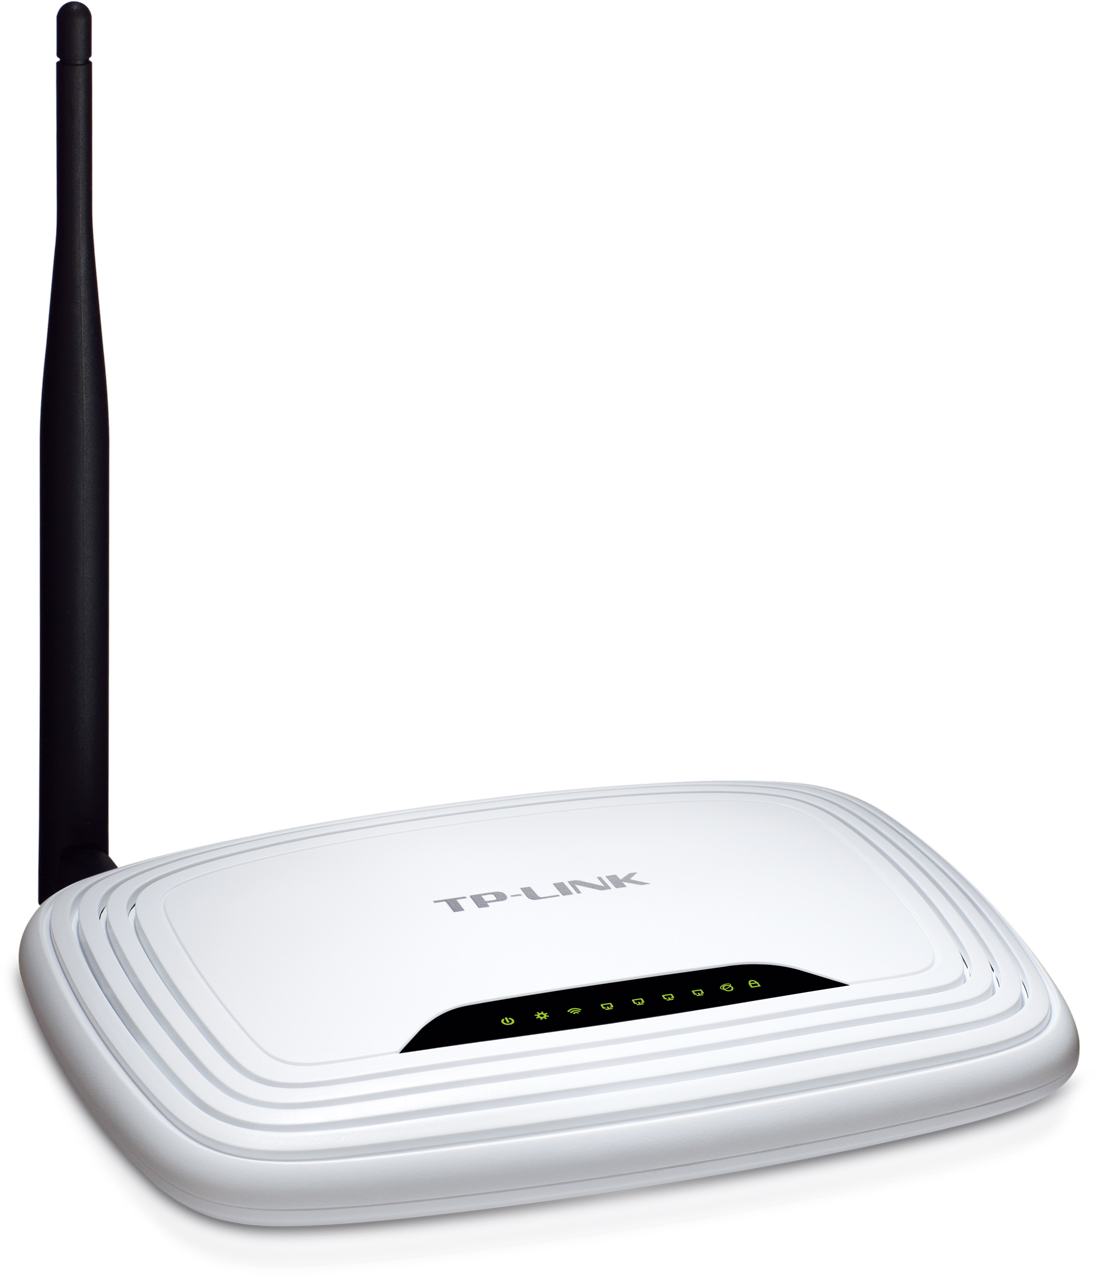
\includegraphics[width=0.2\linewidth]{Pictures/chapter4/router.jpg}
		\caption{TP-LINK TL-WR741ND}
	\end{center}
\end{figure}

To summarize, with its 150Mbps wireless data rate and its advanced WiFi security management (\texttt{WPA/WPA2} encryptions), this router provides a rather good base for our active WiFi monitoring system. But in order to be able to execute our program on that device and get results we had to change its firmware with something not proprietary that we can work with and modulate as we want. This is why we have chosen to replace the original TP-LINK firmware with \texttt{OpenWrt} Linux.

\paragraph*{Limitations}
During the development and the implementation of the active monitoring program we had to deal with some limitations directly induced by the router's hardware specifications.
\begin{description}
	\item [Frequency range]: Since the frequency range of the \texttt{TP-LINK TL-WR741ND} goes from \texttt{2.4GHz} to \texttt{2.4835GHz} we were not able to test connections on the \texttt{5GHz} access points interface. Another limitation this frequency range introduced concerns the \texttt{802.11} protocols. Indeed, the router only supports the \texttt{802.11a, g} and \texttt{n (2.4GHz)} standards. The \texttt{802.11n (5GHz)} is not taken into account.

	\item [Filesystem Disk Space]: The available disk space on which \texttt{OpenWrt} packages can be installed is equal to \texttt{1.1Mo} which is rather limited. Even if we remove all unnecessary packages such as \texttt{Luci}, there is not enough space available in order to install all the required packages the application needs. One implication of that is for the utilization of \texttt{OpenSSL}. Indeed, we provide a fully working encrypted log transmission function but since there was not enough space to install the \texttt{openssl} package we took the decision not to use it in our implementation and use a clear text transmission mechanism instead.
\end{description}

\subsection{OpenWrt}
\texttt{OpenWrt} \cite{openwrt} is a highly extensible GNU/Linux distribution for embedded devices. The particularity of \texttt{OpenWrt} is that it is a full-featured, easily modifiable operating system for routers. Indeed, it offers a fully writable file system and a built-in package manager. Thanks to this package manager, we can install any package we want from a software repository allowing us to customize the device to suit any application. All the restrictions and configurations provided by the vendor within its own firmware installed by default on the router are therefore dropped meaning the device using this distribution can feature functions such as \texttt{SSH} server, \texttt{VPN}, custom \texttt{QoS} and so on.

There are several firmwares available for \texttt{OpenWrt}. We have chosen to use the most recent one, \textit{OpenWrt 12.09 - Attitude Adjustment}, for our active monitoring solution. This ensure a reliable and up-to-date environment for our application.


\subsection{Active WiFi Monitoring Solution}
As detailed above, our active WiFi monitoring solution is based on a \texttt{C} program running on an \texttt{OpenWrt} router. The program uses the \texttt{wpa\_supplicant} API in order to connect to the five different networks of the UCL. During the connection processes, a log file is created and maintained by the program to store important information about the network's behavior. 

In this subsection we first give an overview of \texttt{wpa\_supplicant} and how we use it in our implementation. Then, we explain how our program is structured and what are the key parts that make it work and that make us able to get some insights about the network in real time.

\subsubsection{\texttt{wpa\_supplicant}} %RSN = Robust Security Network
 As defined in \cite{wpa-supplicant}, \texttt{wpa\_supplicant} is a WPA Supplicant for Linux, BSD and Windows with support for WPA and WPA2 (\texttt{IEEE 802.11i/RSN}). Supplicant is the \texttt{IEEE 802.1X/WPA} component that is used in the client stations. It implements key negotiation with a WPA Authenticator and it can optionally control roaming and \texttt{IEEE 802.11} authentication-association of the WLAN driver.

 This supplicant uses portable \texttt{C} code and is divided into several separate files containing independent modules besides from the core part. The core part embedded functionality for controlling the network selection, association and configuration while independent modules include code dealing with \texttt{WPA} (such as key handshake, pre-authentication, etc.), \texttt{EAPOL} and \texttt{EAP} state machines and methods. Also, \texttt{wpa\_supplicant} implements a control interface that we use in our program and that can control the operations of the \texttt{wpa\_supplicant} daemon.

The following figure gives an overview of all the wpa\_supplicant modules and how they interact with each other.

 \begin{figure}[H]
 	\begin{center}
		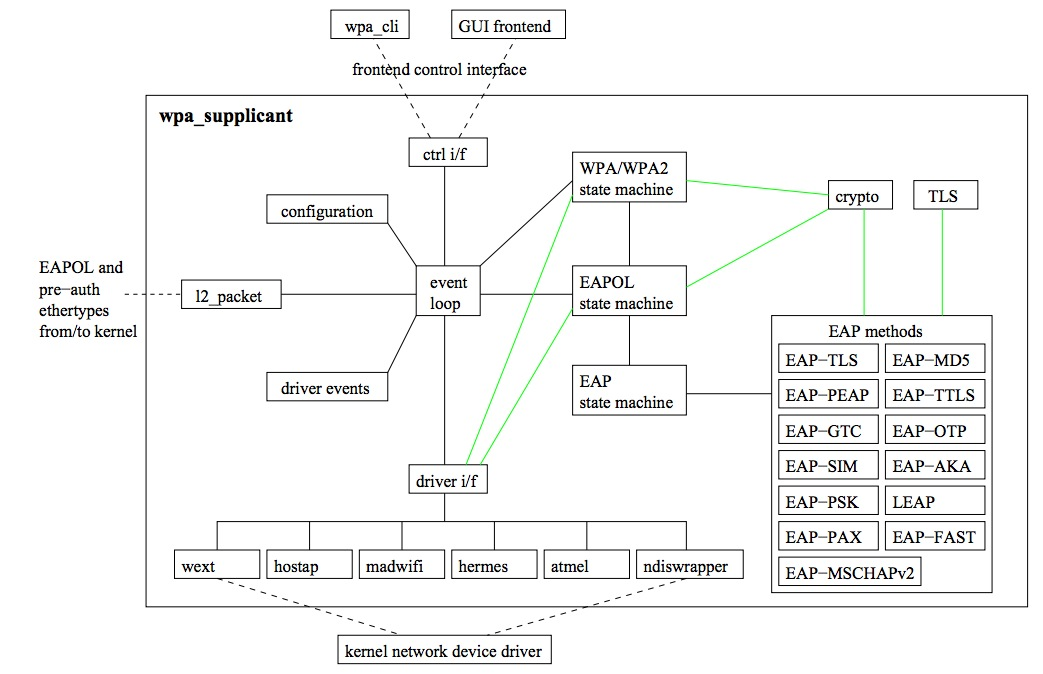
\includegraphics[width=1\linewidth]{Pictures/chapter4/wpa-supplicant-modules.jpg}
		\caption{\texttt{wpa\_supplicant} modules}
	\end{center}
\end{figure}

Within the \texttt{wpa\_supplicant} source package there is a small \texttt{C} file, \texttt{wpa\_ctrl.c}, that provides several functions to facilitate the use of that control interface. We link this file into our program to be able to use that library of functions in order to interact and communicate with \texttt{wpa\_supplicant}. Once that file is linked into our program, we are able to open a connection to the control interface with the \texttt{wpa\_ctrl\_open()} function and we can start sending commands to \texttt{wpa\_supplicant} with the function \texttt{wpa\_ctrl\_request()}. In order to receive messages from the daemon, our program also needs to attach to the control interface using \texttt{wpa\_ctrl\_attach()}.

Several commands can be sent to the \texttt{wpa\_supplicant} daemon but we only use a small selection since most of them are unrelated with our subject of study. Here is the list of the commands we use in our program and their meaning:

\begin{itemize}
	\item[-] \texttt{SCAN}: This command request the daemon to perform a new BSS\footnote{Basic Service Set. The set composed of the access point and the stations in its coverage zone.} scan.

	\item[-] \texttt{SCAN\_RESULTS}: This is used to get the latest scan results. Those results embed details about the bssid, the frequency, the signal level, the flags and the \texttt{SSID} of each network scanned. The message returned has the same syntax as in the following example representing one scan result for each one of the five networks of the UCL.\\

\begin{lstlisting}[frame=single,breaklines=true,caption={Scan results message example}]
bssid / frequency / signal level / flags / ssid
68:86:a7:30:a0:a2	2437	-56	[WPA-EAP-TKIP][WPA2-EAP-CCMP][ESS]	eduroam
00:1e:bd:65:34:73	2462	-55	[WPA-EAP-TKIP][WPA2-EAP-CCMP][ESS]	visiteurs.UCLouvain
00:1e:bd:65:34:71 	2462	-56	[WPA-EAP-TKIP][WPA2-EAP-CCMP][ESS]	student.UCLouvain
68:86:a7:30:a0:a0 	2437	-55	[WPA-EAP-TKIP][WPA2-EAP-CCMP][ESS]	UCLouvain
68:86:a7:30:a0:a4 	2437	-57	[ESS]	UCLouvain-prive
\end{lstlisting}

	\item[-] \texttt{ADD\_NETWORK}: This command adds a new network with an empty configuration. This network is disabled at first and can be configured using the next command. The \texttt{ADD\_NETWORK} command returns a message containing the id of the new network or \texttt{FAIL} on failure. In our case, the program adds five networks at boot for the five networks present within the university's campus.

	\item[-] \texttt{SET\_NETWORK <network id> <variable> <value>}: Once the networks have been added, we are able to configure them using this particular command. The \textit{variable} part of the command uses the same data formats as the standard \texttt{wpa\_supplicant} configuration file. For example, here are the different \texttt{SET\_NETWORK} commands used to configure the \texttt{student.UCLouvain} (with ID=1).\\

\begin{lstlisting}[frame=single,breaklines=true,caption={Configuration of the \texttt{student.UCLouvain} network}]
SET_NETWORK 1 ssid "student.UCLouvain"
SET_NETWORK 1 key_mgmt WPA-EAP
SET_NETWORK 1 eap TTLS
SET_NETWORK 1 identity "login@wifi.uclouvain.be"
SET_NETWORK 1 password "password"
SET_NETWORK 1 ca_cert "etc/wpa_supplicant/chain-radius.pem"
SET_NETWORK 1 pahse2 "auth=PAP"
\end{lstlisting}

	\item[-] \texttt{SELECT\_NETWORK <network id>}: This command asks the \texttt{wpa\_supplicant} daemon to select a special network with the specified ID. When the network is selected, all the others are disabled and the dameon starts the association and authentication phase with the AP in order to establish a connection.

	\item[-] \texttt{DISCONNECT}: This command disconnects the supplicant from the current network.
\end{itemize}

Thanks to those commands our program can control the \texttt{wpa\_supplicant} daemon and is thus able to simulate a typical user's behavior connecting to the networks. More information about \texttt{wpa\_supplicant} can be found inside the developer's guide \cite{wpa-supplicant-devel}.


\subsubsection{Design and Implementation}
In this section we describe the implementation details of our active monitoring program and how it gathers data about the current state of the networks.

The program is composed of two threads that perform different actions. One thread is only dedicated to the \texttt{wpa\_supplicant} control interface and listens to the incoming events sent from that interface. The second thread is dedicated to the connection loop and to the bunch of tests we performed on the network. This second thread is also responsible for sending the log file to the server.

Let's analyse the first thread. The first thing the program does at boot is to start the \texttt{wpa\_supplicant} daemon. To do that, we have created an empty configuration file for the supplicant in order to launch it without starting any connection establishment to the specific network defined in that file. The configuration file contains the following options:\\

\begin{lstlisting}[frame=single,breaklines=true,caption={\texttt{wpa\_supplicant.conf}}]
ctrl_interface=/var/run/wpa_supplicant
eapol_version=1
ap_scan=1
fast_reauth=1
\end{lstlisting}

\par The first parameter asks \texttt{wpa\_supplicant} to open a control interface that is available for external programs to manage the supplicant. The path \texttt{var/run/wpa\_supplicant} is the recommended directory for sockets. 

The second parameter forces the supplicant to use the \texttt{EAPOL} version 1. Version 2 is available but there are many APs that do not handle that version correctly. In order to have a completely working and portable solution we have set the version number to the default value.

The next parameter is about the AP scanning and selection. Three values are possible for that parameter (0, 1 and 2). The value we chose for the program is 1 and it means that it is the supplicant that initiates the scanning and the AP selection. We have decided to set that parameter to the default value 1 because, as for the \texttt{EAPOL} version, we want our program to be used in any situations and infrastructures. The value 0 is generally used for wired networks and the value 2 is used with special drivers and is generally used for ad-hoc networks.

Finally the last parameter is about the \texttt{EAP} fast re-authentication. By default it is enabled for all \texttt{EAP} methods that support it. There is no need to disable this.


The supplicant uses the driver \texttt{nl80211} which is the current standard (the \texttt{wext} driver being deprecated) and uses the \texttt{wlan0} interface. The daemon is started using the following line.\\

\begin{lstlisting}[frame=single,breaklines=true,caption={Starting the \texttt{wpa\_supplicant} daemon}]
system("wpa_supplicant -B -D nl80211 -i wlan0 -c /etc/wpa_supplicant/wpa_supplicant.conf")
\end{lstlisting}

Once the supplicant is launched we open a connection with the control interface using \texttt{wpa\_ctrl\_attach("/var/run/wpa\_supplicant/wlan0")}. That function returns a pointer to the abstract control interface data and is stored inside an internal \texttt{wpa\_ctrl} structure. The next step is to attach the program to the control interface in order to receive messages from that interface. Once the attachment has been performed we start the creation and configuration of the different networks.

That creation is divided into two distinct parts:
\begin{description}
	\item [1) Add the networks]: We use a \texttt{for} loop that adds exactly \texttt{NUM\_OF\_NETWORKS} new networks using the command "\texttt{ADD\_NETWORK}". In our case, we add five networks. Each network has an ID that starts from 0 and that is incremented each time a new network is added.

	\item [2) Configure the networks]: We have implemented a special function \texttt{config\_network()} that configures those previously created networks using the "\texttt{SET\_NETWORK <network id> <variable> <value>}" command. The IDs of the networks, in our case, are the following:
		\begin{itemize}
			\item [-] \texttt{eduroam}: 0
			\item [-] \texttt{UCLouvain}: 1
			\item [-] \texttt{visiteurs.UCLouvain}: 2
			\item [-] \texttt{UCLouvain-prive}: 3
			\item [-] \texttt{student.UCLouvain}: 4
		\end{itemize}
\end{description}

After that creation and configuration phase, the first thread waits for an event from the control interface using the function \texttt{wpa\_ctrl\_recv()}. The event is stored into a buffer and is parsed by the function \texttt{parse\_event()}. Thanks to this function we can retrieve all the important messages sent from the interface and execute the actions required. Our program tracks three types of messages:
\begin{itemize}
	\item \texttt{Trying to associate with <BSSID> (SSID='<SSID>' freq=Frequency)}
	\item \texttt{Associated with <BSSID>}
	\item \texttt{CTRL-EVENT-CONNECTED}
\end{itemize}

This function is also the core part for collecting data that has to be inserted into the log file. Indeed, it is where all the data are stored into structures that will be used later to write the log file. All the information are stored into a set of different structures depending on the type of data. First of all, for each new connection to one of the five networks, there is a main structure, called \texttt{log}, that stores all the information we want to keep for those particular connections. The log structure has six variables.\\

\begin{lstlisting}[frame=single,breaklines=true,caption={Log structure}]
struct log {
	char *date;
	char *ssid;
	struct ap_tried *tried;
	struct ap_connect *connected;
	struct ap_time *time;
	struct check_serv *services;
};
\end{lstlisting}

As we can see, our implementation uses nested structures. Indeed, besides that main structure we also have structures that store all the information about the APs tried during the association phase and the APs the supplicant may have established a connection with on the same network. Each one of these two structures has three variables. First of all the \texttt{BSSID} of the AP the supplicant tried to associate or made a connection with, the number of nodes of the linked list and the next node. The following listings give an overview of those two structures.\\

\begin{lstlisting}[frame=single,breaklines=true,caption={Tried APs structure}]
struct ap_tried {
	char *bssid;
	int num;
	struct ap_tried *next;
};
struct ap_tried *first = NULL;
struct ap_tried *curr = NULL;
\end{lstlisting}\hfill\\\\\\\\

\begin{lstlisting}[frame=single,breaklines=true,caption={Connected APs structure}]
struct ap_connect {
	char *bssid;
	int num;
	struct ap_connect *next;
};
struct ap_connect *first_connect = NULL;
struct ap_connect *curr_connect = NULL;
\end{lstlisting}

We use one more structure in this function that keeps track of the time the daemon took since the start of the association and authentication phase until the connection establishment. We also keep track of the time elapsed in order to get an \texttt{IP} address from the \texttt{DHCP} servers. Those data are stored into the following structure.\\

\begin{lstlisting}[frame=single,breaklines=true,caption={Elapsed time structure}]
struct ap_time {
	struct timeb wpa_time;
	struct timeb dhcp_time;
};
\end{lstlisting}

Let's now describe how the function reacts when it receives one of the three special events from the interface by analyzing each one of those messages.

\begin{description}
	\item[Trying to associate with $<$BSSID$>$ (SSID='$<$SSID$>$' freq=Frequency)]\hfill \\
		As explained before, the first thing the supplicant does when it tries to connect to a network is trying to authenticate and associate with one of the AP that broadcasts the network \texttt{SSID} it wants to connect to. Here is an example of what are all the messages received during a connection establishment to the \texttt{student.UCLouvain} network.\\

\begin{lstlisting}[frame=single,breaklines=true,caption={Example of a trying to authenticate and associate with an AP}]
Successfully initialized wpa_supplicant
wlan0: SME: Trying to authenticate with 00:1e:bd:65:34:71 (SSID='student.UCLouvain' freq=2437 MHz)
wlan0: Trying to associate with 00:1e:bd:65:34:71 (SSID='student.UCLouvain' freq=2437 MHz)
\end{lstlisting}

	As soon as the \texttt{parse\_event()} function receives a "\textit{Trying to associate}" event, it first extracts the \texttt{SSID} of the network from the event. This piece of information is stored into a global variable that will be used later when the log file will be filled. The next thing is to create the first node of the linked \textit{ap\_tried} list if it is the first AP tried for that network, or to add another node to the linked list. In each node, the \texttt{BSSID} of the AP is stored. Also, the number of nodes, \texttt{num}, is incremented.

	\item[Associated with $<$BSSID$>$]\hfill \\
	Once the association with the AP is completed, the interface sends an association event. Let's continue the example above with the connection to the \texttt{student.UCLouvain} network.\\

\begin{lstlisting}[frame=single,breaklines=true,caption={Example of a association with an AP}]
wlan0: Trying to associate with 00:1e:bd:65:34:71 (SSID='student.UCLouvain' freq=2437 MHz)
wlan0: Associated with 00:1e:bd:65:34:71
\end{lstlisting}
In that case, we extract the \texttt{BSSID} of the AP that the daemon is associated with and we store it directly in our main log structure.

	\item[CTRL-EVENT-CONNECTED]\hfill \\
	This event means that the daemon is now connected to the AP after the \texttt{EAP} authentication has been performed. These are the final messages received during the connection establishment of our example.\\

\begin{lstlisting}[frame=single,breaklines=true,caption={Example of a connection to the \texttt{student.UCLouvain} network}]
wlan0: Associated with 00:1e:bd:65:34:71
wlan0: CTRL-EVENT-EAP-STARTED EAP authentication started
wlan0: CTRL-EVENT-EAP-PROPOSED-METHOD vendor=0 method=21
wlan0: CTRL-EVENT-EAP-METHOD EAP vendor 0 method 21 (TTLS) selected
wlan0: CTRL-EVENT-EAP-SUCCESS EAP authentication completed successfully
wlan0: WPA: Key negotiation completed with 00:1e:bd:65:34:71 [PTK=CCMP GTK=TKIP]
wlan0: CTRL-EVENT-CONNECTED - Connection to 00:1e:bd:65:34:71 completed (auth) [id=0 id_str=]
\end{lstlisting}

When the function receives this event, there are several actions that are executed. First, the \texttt{BSSID} is extracted from the event and, as for the \textit{Trying to associate} event, the linked ap\_connect list is created or extended. Besides that, the time structure is also filled with \texttt{wpa\_supplicant} connection time and \texttt{DHCP} time. Basically, we evaluate the time taken by \texttt{wpa\_supplicant} to get a connection by starting a timer at the time our program requests a connection with one of the network and we stop the timer when this special event is received. Same for \texttt{DHCP}. We start the timer just after the reception of the event and before starting the \texttt{DHCP} process by using the command \texttt{system("udhcpc -i wlan0")}. As soon as the supplicant has received an \texttt{IP} address we stop the timer. Those time information are stored directly into the ap\_time structure that is nested inside the log structure.

\end{description}

Thanks to that \texttt{parse\_event()} function, complete data about the \texttt{SSID} of the network, the list of all APs that the supplicant tried to associate with, the ones it has established a connection with and the time duration of all those processes are already stored into our main structure.


Let's now analyse the second thread. We can divide the work of this thread into four categories. It handles the main connection loop, performs a scan, checks the availability of the services and, most importantly, fills the log file and sends it to our server. 

\begin{description}
	\item[Connection loop]: This is the core part of our monitoring system. Indeed, the loop embeds the key processes of our tool.The choices we made for the loop are the following: first, the program performs a scan of the networks available around the router and the results are inserted inside the log file. Then the connection loop begins and for each network, the supplicant tries to establish a connection. Once the connection is established, the availability of a selection of services is tested in order to see if a user can access to them when he is connected to that particular network. Finally the supplicant is disconnected from the current network and the process restarts for the next one. After a selected number of loops (5 by default), the log file is closed and sent to the server. A new file is then opened and the loop starts again. The following pseudo-code gives a better understanding of how the loop works.

\begin{lstlisting}[frame=single,breaklines=true,caption={Connection loop pseudo-code}]
WHILE 1
	CALL scan
	FOR each network
		CALL execute_action with ACTION_CONNECT, network
		CALL services_loop
		CALL log_event with LOG_PRINT_STRUCT
		IF number of loops = NUM_OF_LOOPS-1 AND network = last THEN
			CALL fclose with file
			CALL send_log
			CALL fopen with file path
			Set number of loops to 0
		ELSE
			CALL execute_action with ACTION_DISCONNECT
			INCREMENT number of loops
		ENDIF
	ENDFOR
\end{lstlisting}

	\item[Scan]: At the beginning of every connection loop, the program performs a scan of all the available networks and keeps the results in a special structure in order to include them into the log file afterwards. Thanks to those information, we have a more detailed overview of the router's surrounding environment and what are the APs specifications there. This process is handled by the function \texttt{scan()}. In order to perform this scan we first send the command \texttt{SCAN} to the interface and then we collect the results into a buffer by sending the command \texttt{SCAN\_RESULTS}. The results are stored into a custom structure containing seven variables. The structure is the following.\\

\begin{lstlisting}[frame=single,breaklines=true,caption={\texttt{scan\_results} structure}]
struct scan_results {
	char *bssid;
	char *freq;
	char *signal;
	char *flags;
	char *ssid;
	int num;
	struct scan_results *next
};
struct scan_results *first_scan = NULL;
struct scan_results *curr_scan = NULL;
\end{lstlisting}
	
	For each line of the scan results we extract the \texttt{BSSID}, the frequency, the signal, the flags and the \texttt{SSID} of the network the AP broadcasts. All this data is stored into one node and, as for the other linked list, the node is either the first one or is added to the others. Once all the results from the buffer have been parsed and inserted into the linked list, the program automatically adds the scan results into the log file in which we have decide to keep only the \textit{bssid}, \textit{freq}, \textit{signal} and \textit{signal} variables.

	\item[Services checking process]: This is a special feature we have implemented in our monitoring tool. The idea is to emulate the behavior of a lambda user that connects to one of the networks. We verify that a list of services is reachable once connected to the network. The process is divided in two parts. First we check if the two \texttt{DNS} servers (\texttt{130.104.1.1} and \texttt{130.104.1.2}) are accessible. To do that we query the two servers by forging and sending a special \texttt{DNS} query packet and we analyse the response received. After that we perform an reachability check on a list of selected websites. We check the ten most visited websites in the world, according to Alexa\footnote{http://www.alexa.com/topsites} (we made sure to remove the Chinese ones), and we add the main UCL's websites the clients often visit. Here is the complete list:
	\begin{itemize}
		\item[-] \texttt{DNS} (\texttt{130.104.1.1})
		\item[-] \texttt{DNS} (\texttt{130.104.1.2})
		\item[-] google.be
		\item[-] facebook.com
		\item[-] youtube.com
		\item[-] be.yahoo.com
		\item[-] en.wikipedia.org
		\item[-] twitter.com
		\item[-] amazon.fr
		\item[-] live.com
		\item[-] linkedin.com
		\item[-] blogspot.com
		\item[-] smtp.gmail.com
		\item[-] github.com
		\item[-] uclouvain.be
		\item[-] icampus.uclouvain.be
		\item[-] moodleucl.uclouvain.be
		\item[-] bib.sipr.ucl.ac.be
		\item[-] horaire.sgsi.ucl.ac.be
		\item[-] studssh.info.ucl.ac.be
	\end{itemize}

	Concerning the availability check for the list of websites, we create a socket and try to connect to the remote server through this socket. All the reachability information are stored into a special structure called \texttt{check\_serv}.

	\item[Log file]: Finally, all the data collected during the connection loop process and stored into the different structures are inserted into the log file. We use a \texttt{JSON} syntax for the log file since we already use a \texttt{JSON} parser on our server. Thanks to this design the portability is maintained and enhanced. We have defined several conventions for our log file that is divided into several parts. As an introduction we print the date on which the log file was started and the \texttt{MAC} address of the router to help the server distinguish between all the log files he may receive from various probes. Then first we have all the information about the scan results. After that we find all the data regarding the connection loop. This part is divided into sections where each one of them represents one network and contains all the details about it. At the end, we find all the information about the reachability and availability tests made on the set of services ("0" meaning that the service is not reachable and "1" meaning the opposite). Here is a small example of a log file, with only one scan result, one connection and the services, our server receives from the probe for readability.\\


\begin{lstlisting}[frame=single,breaklines=true,caption={Small log file example}]
{
	"date": "2014/05/23 14:54:17",
	"mac": "a0:f3:c1:36:87:58",
	"log": [
		"scan": 
		[
			{
				"bssid": "00:1e:bd:65:34:71",
				"frequency": "2462",
				"signal": "-56",
				"ssid": "student.UCLouvain"
			}
		],
		"connections": 
		[
			{
				"date": "2014/5/23 14:54:18",
				"ssid": "student.UCLouvain",
				"tried": 
				[ 
					"00:1e:bd:65:34:71"
				],
				"connected": 
				[ 
					"00:1e:bd:65:34:71"
				],
				"time": 
				{
					"wpa_supplicant": "2sec 35ms",
					"dhcp": "1sec 12ms",
				},
				"services":
				{
					"google.be": "1",
					...
					"studssh.info.ucl.ac.be": "1"
				}
			}
		]
	]
}
	\end{lstlisting}
\end{description}


\section{Communication between Server and Probes}
The probes and the server have to exchange information. As we wanted to create a modular tool, we have chosen to encrypt all the data sent between the server and the probes. If the active monitoring device captures sensible contents, no security vulnerabilities like \emph{eavesdropping} or \emph{man-in-the-middle attack} can be accepted.
The first constraint that appeared was the weak computation power of the probes. In consequence, we had to keep the encryption as easy to perform as possible. So, we have dived into \emph{symmetric cryptographic} techniques. Also, since there may have several probes working at the same time, it could be difficult to manage and exchange the keys. Asymmetric cryptography can fix that problem. Finally our choice was to take the best part of both worlds and implement a protocol using hybrid encryption.
In definitive, we used \texttt{RSA} and \texttt{AES} encryption together.

\subsection{RSA}
\texttt{RSA}\footnote{\url{http://www.google.com/patents/US4405829}} is one of the most used public-key cryptosystem. The main advantage against symmetric cryptography is that the public key used for the encryption can be known by everybody and so make the problem of key exchange a lot easier.
%\begin{enumerate}
%\item Alice give her public key to Bob.
%\item Bob wants to transmit a encrypted message to Alice. He uses the Alice's \emph{public key} to encrypt the message.
%\item Bob sends his message to Alice. Even if people intercept the transmission and have the public key, they couldn't decrypt it.
%\item Alice receives the message and decrypt it with her private key which she have kept secret.
%\end{enumerate}

The key is 2048 bits long and each entity has its own pair of keys (i.e. the server and each probe). The server will know which are the authorized probes by having their private keys and it will use them to encrypt the \texttt{AES} key.
The main drawback of such encryption is that the computations are quite heavy to perform, which is against our previous requirement. That is why we only use it to encrypt and exchange a symmetric key that will be used for the data exchange.

\subsection{AES}
The symmetric algorithm we use is the \texttt{AES}\footnote{Advanced Encryption Standard}. We chose a key size of 256 bits which is quite suitable for our utilization. The idea is to permute the bits of the message using the key. The operations performed are lighter than the ones in \texttt{RSA} and so it is more adapted to be used on the probes.


\subsection{Transaction Protocol}
To be correct, the exchanges made between the probes and the server require a protocol well defined and respected by the two parts. As mentioned earlier, the server knows the public key of every probe in advance and can use them to encrypt the \texttt{AES} key. The next step is the transmission of that key as well as the \emph{Initialization Vector}. When the two parts own the \emph{symmetric} key, the exchange can be encrypted with light computation. The data are sent to the server and it can parse them and store the information into the database.
% Put diagramme sequence

\paragraph*{OpenSSL}
On the \texttt{OpenWRT} router, the encryption is realized by the \texttt{OpenSSL} library. These methods offers abstraction to use \texttt{RSA} and \texttt{AES}. As a reminder, the functions are implemented but due to the hardware limitations of the router they are not deployed.

\paragraph*{PyCrypto} Since the server is written in \texttt{Python}, we used the \texttt{PyCrypto} module that offers a wrapper for the cryptographic functions required by our protocol.

\section{Web Interface}
For our user interface, we have chosen to use the \emph{Bootstrap} framework\footnote{http://getbootstrap.com/}. It is widely use and well documented. It allows to quickly develop intuitive and responsive interfaces and is automatically compatible with mobile devices. As we focus mainly on the back-end of our system, we needed to be able to build the interface as quickly as possible but still with quality. That is why we have coupled the \texttt{Django} templates system with that framework. Finally, we complete them with the \emph{Google Chart} library. A more exhaustive explanation of those technologies is available in section \texttt{4.6}.


\section{Deployment}
Concerning the deployment of our monitoring tool, we had a dedicated server to host our data. This system was quite limited in order to efficiently serve all the requests. The server has a hard drive of \texttt{300GB} which is quite enough to store all the information gathered by \texttt{NetwObserver} during the deployment and the test phases. On the other hand, the memory available is only \texttt{1GB} which is not enough to ensure an efficient handling of the users requests.

\subsection{Apache 2}
Since the interface of the system is composed of web pages, all the \texttt{HTTP} requests are handled by Apache 2\footnote{http://httpd.apache.org/}. A lot of documentation about this \texttt{HTTP} server is available online since it is the most widely used. That is the main reason why we decided to choose it.

\subsection{Module WSGI}
This \texttt{Apache} module is a module able to interpret some \texttt{Python} code. As said before, we chose \texttt{Django} as a framework for our application, and in consequence executing \texttt{Python} code is an important requirement. Something important to mention about the installation is that the code is written in \texttt{Python3.3} and not in the version 2. That forced us to be careful during the installation as the default \texttt{Python} interpreter in most system is the \texttt{2.6}. In definitive, we have to compile the module \texttt{WSGI} with the specification of the right interpreter.

\subsection{Celery}
\texttt{Celery}\footnote{http://www.celeryproject.org/} is a distributed task queue. It allows to create asynchronous jobs handled by several \emph{workers}. Concretely, a worker is a external thread that receives tasks to accomplish. The main drawback of \texttt{Apache 2} is that it is quite complicated to generate and manage daemons running in background constantly or at given intervals. As a turn-around, we have connected our system to \texttt{Celery}. It helps us to manage more efficiently the concurrent elements of the application. Our server has a small memory capacity and a poor computation power and in consequences we must manage and organize the utilization of those resources. This module has two main component: the \emph{workers} and the \emph{scheduler}.

\subsubsection*{The Workers}
In \texttt{Celery}, we can define the number of threads working on the tasks. By adapting this number, we can tune the allocation of the processor. For example, when we execute a set of \texttt{SNMP} requests, it may require a large part of the available resources. Each one of these sets of requests are executed at different intervals and can sometime overlap. When that situation occurs, the server can experience heavy computation processes and may have trouble to handle all the requests generated by the users. That is why we define a fixed number of workers and a queue. Each task waits in the queue until a slot is available. The main drawback of such an architecture is that the exact time when the job starts and is effectively done remains undetermined. Even if it can be really problematic in some contexts, it is not the case in our system. Indeed, in our system we have either a daemon that runs endlessly or we have tasks, such as \texttt{SNMP} requests, that have to be executed. In either case, this is not a real issue since they do not have precise time requirements. 


\subsubsection*{The Scheduler}
The scheduler in \texttt{Celery} is called \emph{beat} and its only responsibility is to send the \emph{periodic tasks} to the workers. It knows the path of the application in which we have defined the tasks and the related intervals. \texttt{Celery beat} gathers those intervals and fires the tasks accordingly. The main thing to take into account about the scheduler is the fact that it launches the tasks \textbf{exactly} at each interval. If we imagine a task that takes between 4 and 5 minutes to perform and an interval of 10 minutes, there can be moments where two instances of that tasks overlap. Indeed, if all the workers are occupied and the first instance only starts after 8 minutes, the second task will start two minutes later while the first one is still running. Here again, such consideration have been taken care of and the data are stored with a time stamp or linked to an already existing entity. Since the intervals vary from 20 minutes to 2 hours whilst the results are being analysed, the impact is quite reduced. 

\section{Extensions and Portability}

In this section we give some further details about the overall portability and modularity of our application and how extensions can be added to the source code in order to provide other features.

\subsection{NetwObserver}
We focus on making our code as modular and extensible as possible. Each gatherer and analyser are implemented to be easily understood by an external developer. To illustrate that we will take the example of adding an extension to this gatherer and we proceed it through each part of our system.

\paragraph*{Gathering a New SNMP Data} For our example, we will add the monitoring of the percentage of time spent by an interface to send and receive data. The first step is to determine to way of gathering those information. They are both easily available using the \texttt{SNMP} protocol.

\begin{tabular}{|r l|}
\hline
\textbf{Object} & \texttt{bsnAPIfLoadRxUtilization} \\
\textbf{Description} & \parbox{11cm}{This is the percentage of time the Airespace AP receiver is busy operating on packets. It is a number from 0-100 representing a load from 0 to 1.} \\
\textbf{OID} & 1.3.6.1.4.1.14179.2.2.13.1.1 \\
\textbf{MIB} & AIRESPACE-WIRELESS-MIB \\
\hline
\end{tabular}

\begin{tabular}{|r l|}
\hline
\textbf{Object} & \texttt{bsnAPIfLoadTxUtilization} \\
\textbf{Description} & \parbox{11cm}{This is the percentage of time the Airespace AP transmitter is busy operating on packets. It is a number from 0-100 representing a load from 0 to 1.} \\
\textbf{OID} & 1.3.6.1.4.1.14179.2.2.13.1.2 \\
\textbf{MIB} & AIRESPACE-WIRELESS-MIB \\
\hline
\end{tabular}

Once we have a clear idea of how to gatherer the data, we use the abstractions of the system to teach it how to collect them. Since those values are available for each interface of each access point, we use the method \texttt{walkByInterface()} that is implemented to collect such data and aggregate them by AP. We continue our example by defining our two new methods.\\

\begin{lstlisting}[language=Python, frame=single,breaklines=true,caption={Adding the two new methods}]
def getAPIfLoadRxUtilization(ip, port=settings.SNMPPORT, community=settings.SNMPCOMMUNITY, ap=''):
	return walkByInterface(ip=ip, oib='1.3.6.1.4.1.14179.2.2.13.1.1', port=port, community=community)

def getAPIfLoadTxUtilization(ip, port=settings.SNMPPORT, community=settings.SNMPCOMMUNITY, ap=''):
	return walkByInterface(ip=ip, oib='1.3.6.1.4.1.14179.2.2.13.1.2' + ap, port=port, community=community)
\end{lstlisting}

Once the methods are defined, we can finally add them to the \texttt{getAllAP()} method that manages the \texttt{SNMP} requests. This method executes each one of the request and crosses the data with the ones already gathered. Concretely, we add two calls to the \texttt{getIfSnapshotData()} method in the \texttt{getAllAP()} method. It performs a snapshot of the data and saves them into the database.\\

\begin{lstlisting}[language=Python,frame=single,breaklines=true,caption={Adding two calls to \texttt{getIfSnapshotData()}}]
getIfSnapshotData(resultIfSnapshot, 'txUtilization', getAPIfLoadTxUtilization,ip=ip, port=port, community=community)
getIfSnapshotData(resultIfSnapshot, 'rxUtilization', getAPIfLoadRxUtilization,ip=ip, port=port, community=community)
\end{lstlisting}

At this step, the data are already recorded at each periodical execution of the \emph{SNMP} requests. They are available to define new analysis.

\paragraph*{Aggregation} When the data are available, we need to aggregate them to get a representation of their evolution throughout the days. In our implementation, the system aggregates a number of snapshots and takes the maximum or computes the average. For our data, we have chosen to take the maximum to be able to spot the peak of activity. For this step, we have nothing to do. Indeed, the \texttt{getIfData()} defined in the \texttt{analyse.computation.aggregator} module takes into account the new data once they are available.

\paragraph*{Interface} The interface is based on the \texttt{Django} templates. An interface is defined by blocks. Each block is defined once and can be inherited by several interfaces. This mechanism is possible thanks to the utilization of specific tags in the \texttt{HTML} code. We did not have implemented that system and a complete documentation is available online\footnote{https://docs.djangoproject.com/en/1.6/ref/templates/}. 

The graphs are generated by the Google Chart library\footnote{https://developers.google.com/chart/} that allows to generate interactive graphs very easily. Since we use this library with the \texttt{Django} templates, the definitions of the graphs become really easy as we are able to access the aggregated value directly. The \texttt{HTML} tags are put between brackets and allows to generate dynamically the Javascript scripts. In our example, a graph is generated for each interface (\texttt{\{\%for i in interfaceData\%\}}) and the data are added directly by iterating on the aggregated values (\texttt{\{\%for log in i.data\%\}}). The last step is simply some design using \texttt{HTML} and \texttt{CSS}.\\

\begin{lstlisting}[language=Python, frame=single,breaklines=true,caption={Example of Graph definition}]

google.setOnLoadCallback(drawInterface{{forloop.counter0}}Chart);
function drawInterface{{forloop.counter0}}Chart() {
		
	var data = google.visualization.arrayToDataTable([
		  ['Time', 'Clients', 'Clients with Poor SNR', 'Channel Utilization'],
		  
		  [new Date({{log.date.year}},{{log.date.month}}-1,{{log.date.day}},{{log.date.hour}},{{log.date.minute}},{{log.date.second}}), {{log.data.rxUtilization}} , {{log.data.txUtilization}}],
		  
		]);

	var options = {
		title: 'Transmitter and Receiver Occupation',
	};

	var chart = new google.visualization.LineChart(document.getElementById('interface{{forloop.counter0}}chart_div'));
		chart.draw(data, options);
}


\end{lstlisting}

\subsection{Probe}
The active monitoring program has been designed to work only with the UCL's wireless network. Yet some additions and modifications of the source code can be realized in order to extend it. To illustrate that, we detail two possibles extensions. First, adding a new network to monitor and second, adding a new service to check. 

The tricky part of working with \texttt{OpenWrt} is the compilation phase. Indeed, if we want our program to run on the router, we have to \textit{cross compile} it. This is due to the fact that the router does not offer enough memory space in order to directly install the \texttt{C} compiler and to compile the code natively. Also, the router uses a different architecture than we do when developing the program. In our case, the router has a \texttt{MIPS} architecture. This is why the code needs to be cross compiled in order to run on the router. Details about the cross compilation can be found in \cite{crosscompile}.

\subsubsection*{Adding a new network}
Let's take a test network for this example. The specifications of the new network are the following.

\begin{itemize}
	\item [-] \texttt{SSID}: test.UCLouvain
	\item [–] Key Management: \texttt{WPA-EAP}
	\item [-] \texttt{EAP}-Method: \texttt{TTLS}
	\item [-] Login: test@wifi.uclouvain.be
	\item [-] Password: passwd
	\item [-] Inner authentication: \texttt{PAP}
\end{itemize}

The first thing to do is to increment the global variable \texttt{NUM\_OF\_NETWORKS} since it stores the number of networks used throughout the execution of the application.\\

\begin{lstlisting}[frame=single,breaklines=true]
#define NUM_OF_NETWORKS 6
\end{lstlisting}

The final step is to add the network specifications in the \texttt{create\_networks()} function. The network will be configured with the others when the program starts. Here is the line to add to the function.\\

\begin{lstlisting}[frame=single,breaklines=true]
config_network(5, "test.UCLouvain", "WPA-EAP", "TTLS", NULL, "test@wifi.uclouvain.be", "passwd", "/etc/wpa_supplicant/chain-radius.pem", NULL, "auth=PAP");
\end{lstlisting}

As we can see, it is very easy to add a network. If we wanted to delete one of the network, we would have realized the exact opposite. First decrement the global variable and then delete the line responsible for configuring the network we want to remove (making sure to update the first parameter of the other \texttt{config\_network()} function calls (i.e. the IDs of the other networks) accordingly if necessary).


\subsection*{Adding a new service}
As explained earlier, we have provided a selection of 18 services for this application. But more services can be easily added to the check list. Let's say we want to add the website "\texttt{http://foditic.info.ucl.ac.be/}" to the list. Here are the steps that need to be fulfilled in order to check the availability of this website as well.

First, we need to add a variable in the \texttt{check\_serv} structure that will store the result of the socket connection test. This structure is located into the header file \texttt{wifi\_monitoring.h}.\\

\begin{lstlisting}[frame=single,breaklines=true]
struct check_serv {
	char *DNS_1;
	...
	char *studssh;
	char *foditic;
};
\end{lstlisting}

Then we have to, first, allocate memory to this new variable and then add the call to the function that tests the services. The function \texttt{services\_loop()}, located in the main \texttt{wifi\_monitoring.c}, takes two arguments: the address and the port for the connection.\\

\begin{lstlisting}[frame=single,breaklines=true]
static void services_loop() {
	...
	ptr->studssh = malloc(1);
	ptr->foditic = malloc(1);
	...
	if(checkService("studssh.info.ucl.ac.be", "22") == 0)
		strcpy(ptr->studssh, "1");
	else
		strcpy(ptr->studssh, "0");

	if(checkService("foditic.info.ucl.ac.be", "80") == 0)
		strcpy(ptr->studssh, "1");
	else
		strcpy(ptr->studssh, "0");
}
\end{lstlisting}

The last step consists of inserting the new collected information into the log file. To do that, we simply have to add a line into the function \texttt{log\_event()} also located in the main \texttt{wpa\_supplicant.c} file. Notice that we have to add a comma at then end of the previous last line in order to respect the \texttt{JSON} syntax and for our new log file to be parsed correctly by the server.\\

\begin{lstlisting}[frame=single,breaklines=true]
static void log_event(enum log_events log, const char *arg) {
	case LOG_PRINT_STRUCT: {
		...
		fprintf(f, "\"studssh.info.uc.ac.be\": \"%s\",\n", log_struct->services->studssh);
		fprintf(f, "\"foditic.info.ucl.ac.be\": \"%s\"\n", log_struct->services->foditic);
		fprintf(f, "}\n");
	}
	break;
}
\end{lstlisting}


\section{Summary}
This chapter reviewed the whole implementation design and deployment phase of our wireless monitoring tool. Precise information about the components of the system, \texttt{NetwObserver}, were detailed and discussed throughout this chapter. With this better understanding of how the application works we can, in the following chapters, examine the results collected during the deployment phase. 